%-*-coding: utf-8-*-

\chapter{Обзор предметной области}

\section{Вспомогательные понятия}

\subsection{Векторное представление слов}
Векторное представление слова (word embedding)[2]~--- параметризованное отображение слова на пространство большой размерности $R^d$. Такое представление сохраняет семантические отношения между словами. Причем похожим словам сопоставляются близкие по некоторой метрике вектора, а различным ~--- удаленные друг от друга.

Векторное представление слов либо обучают <<с нуля>> вместе с основной моделью, либо берут за основу предобученные на достаточно большом корпусе текстовых данных. Наиболее крупные корпусы векторных представлений это word2vec, а также GloVe, которые также будут использоваться в данной работе.

\todo{Визуализация Word Embedding}

\subsection{Дерево синтаксического разбора предложения}
\todo{Написать тут}

\section{Классификация}

Классификация ~-- один из разделов машинного обучения, посвященный решению
задачи классификации.

\subsection{Задача классификации}

Задача классификации~--- имеется множество объектов, каждый из которых принадлежит
к какому-то классу, количество классов чаще всего ограничено.
Существует обучающая выборка~--- множество объектов, метки
класса которых нам известны. Классовая принадлежность остальных объектов
неизвестна. Задача заключается в построении алгоритма, способного
классифицировать (присвоить метку класса) произвольный объект из исходного множества.

Формально, $X$~--- множество объектов, $Y$~--- множество классов,
существует отношение $y* : X \rightarrow Y$, заданное только для обучающей выборки.
Необходимо построить такой алгоритм $a: X \rightarrow Y$, способный для произвольного
$x \in X$ найти $y \in Y$.	

\section{Численная оценка качества классификации}

\subsection{Accuracy}
Accuracy~--- точность классификации. Самый простой способ оценки эффективности классификатора.
$$Accuracy =\frac{P}{N}$$
$P$~--- количество верно классифицированных объектов\\
$N$~--- количество объектов в выборке

\section{Обзор существующих решений}

В данной главе будут приведены существующие решения задачи sentence modelling, для сравнения с предложенным решением.

\subsection{Paragraph Vector}

\todo{BoW}

Целью подхода Paragraph Vector является сопоставление вещественного вектора в $R^d$ последовательности слов произвольной длины: предложению, абзацу или даже документу.
Paragraph Vector учитывает семантический контекст текста на котором он получен.

Параметрами Paragraph Vector являются: вещественная матрица $W$~--- векторное представление слов словаря текстового корпуса, а также вещественная матрица $D$~--- векторное представление абзацев корпуса. Метод пытается предсказать следующее слово в абзаце, опираясь на векторное представление данного абзаца, а также слов из абзаца, смежных с предсказываемым словом, то есть находящихся в одном контексте с ним.

\begin{figure}[h]
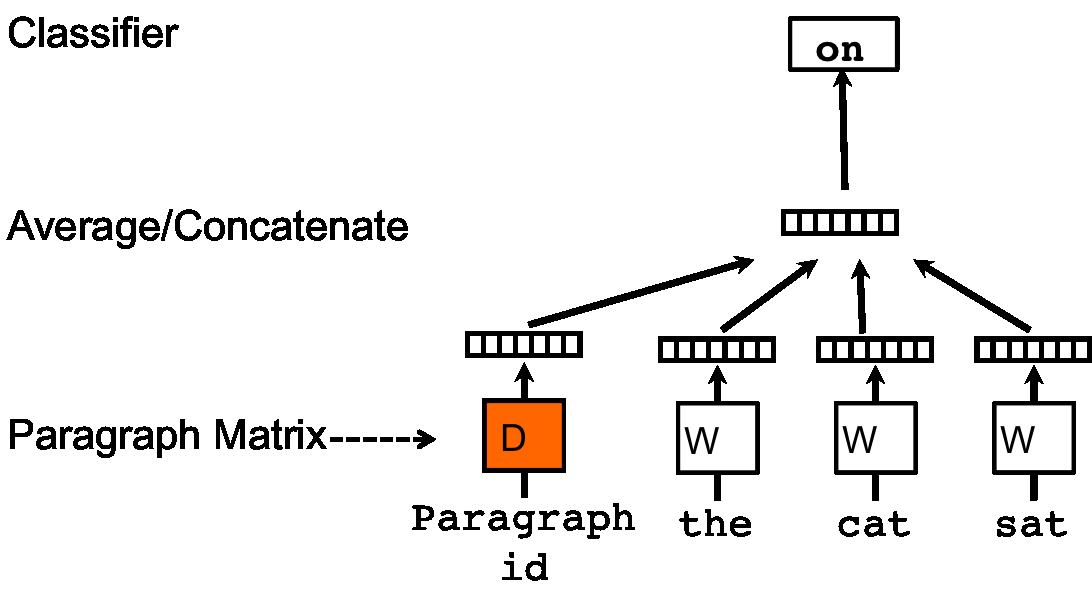
\includegraphics[scale=0.4]{par_vec}
\caption{\textbf{Paragraph Vector}}
\label{fig:par_vec}
\end{figure}

\subsection{Рекурсивные нейронные сети}
Основным инструментом для обработки текстов являются так называемые \emph{рекурсивные нейронные сети}(РНС)[статьи].

Рекурсивные нейронные сети предназначены для обработки последовательных данных, таких как звук и текст. В традиционных нейронных сетях все входы считаются независимыми друг от друга, но для многих задач это не так, и такой подход не учитывает много информации о структуре данных.

Рекурсивные нейронные сети принимают (РНС) слова последовательности поочереди, сохраняя внутри себя контекст уже принятого текста. Рекурсивными они называются потому что выполняют одну и ту же задачу для каждого элемента последовательности (а конкретно для каждого слова в тексте). Они достаточно хорошо отражают процесс восприятия информации человеком: после того как мы прочли начало предложение, в нашей голове уже сформировался некоторый контекст, и следующее слово обрабатывается нами с учетом уже прочитанной информации, а не воспринимается с чистого листа.

\begin{figure}[h]
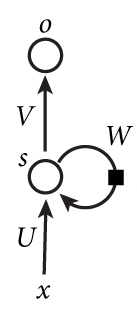
\includegraphics[scale=0.7]{rnn}
\caption{\textbf{РНС}}
\label{fig:rnn}
\end{figure}

\begin{figure}[h]
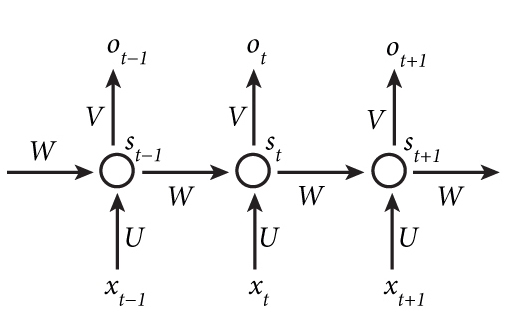
\includegraphics[scale=0.7]{rnn-unfold}
\caption{\textbf{РНС в развернутом виде}}
\label{fig:rnn-unfold}
\end{figure}

\noindent $U, W, V$~--- параметры РНС сети\\
$x_t$~--- вектор, соответствующий слову $t$ \\
$s_t$~--- информация о первых $t$ словах \\
$o_t$~--- выходной вектор

Хотя РНС является достаточно мощной моделью, у нее есть ряд недостатков, самый большой из которых~--- это так называемая <<проблема стирания градиента>>. Суть ее заключается в том, что РНС не может запоминать контекст в длинных последовательностях слов. Поэтому на смену РНС была изобретена другая архитектура РНС, под названием \emph{долгая краткосрочная память} (ДКП) (от англ. Long Short Term Memory или LSTM), которая решает эту проблему[статья].

\begin{figure}[h]
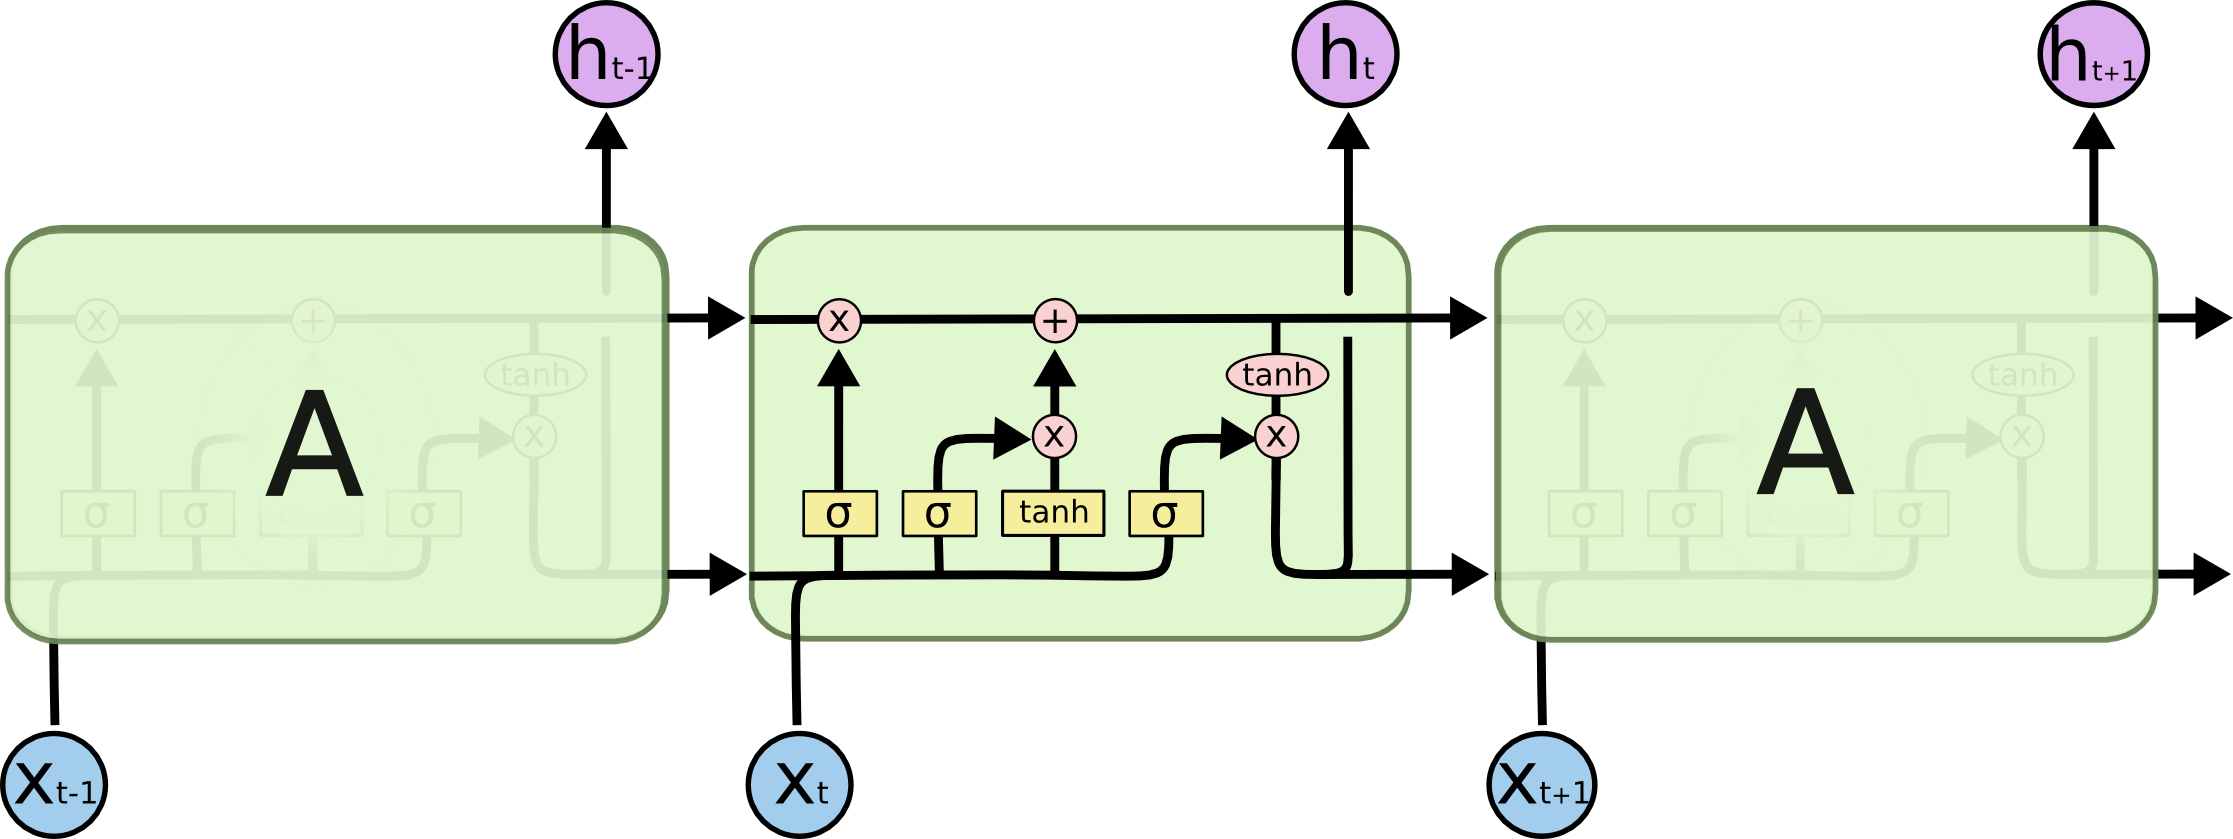
\includegraphics[scale=0.5]{lstm}
\caption{\textbf{Долгая краткосрочная память}}
\label{fig:lstm}
\end{figure}

Таким образом, на вход ДКП подается предложение, и используется последний выходной вектор как векторное представление для задачи sentiment modelling [статья].

\subsection{Сверточная нейронная сеть}
Сверточная нейронная сеть (СНС)~--- успешно показала себя в обработке и анализе изображений.[статья] Они работают подобно тому, как происходит распознавание образов в головной коре человека. СНС состоят из нескольких слоев, каждый из которых детектирует некоторые визуальные признаки изображения, такие как прямые линии, окружности. Признаки с предыдущего слоя используются для формирования более высокоуровневых визуальных признаков.

Преимуществом СНС является выделение локалных пространственных признаков [статья]. В контексте изображений это означает, что визуальные признаки локализуются сначала на неболших квадратах, а далее объединяются в большие фигуры.

Оказывается, данный плюс можно использовать и в задаче sentiment modelling, если рассмотреть слова предложения как вектора некоторой размерности. Тогда если в предложении $n$ слов, 
и размерность векторного представления слова $d$, получаем матрицу $n \times d$, 
которую можно трактовать как изображение и применить к нему сверточную нейронную сеть.[статья].

\begin{figure}[h]
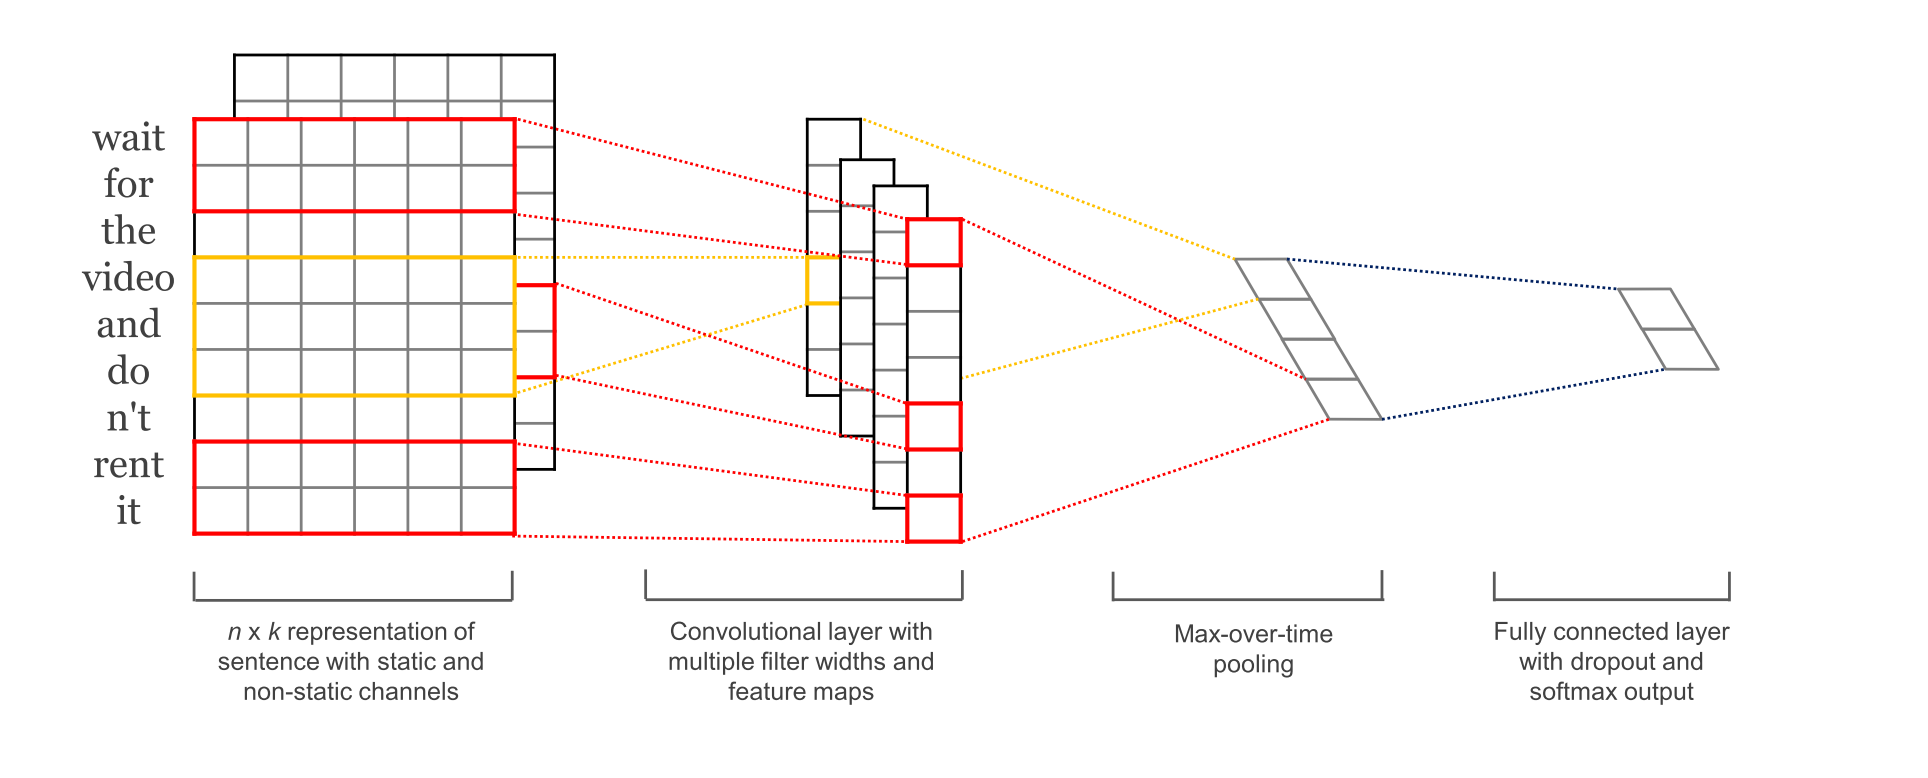
\includegraphics[scale=0.55]{cnn}
\caption{\textbf{СНС для предложения}}
\label{fig:cnn}
\end{figure}

\subsection{Рекурсивная тензорная нейронная сеть}
Еще одним важным подходом к решению задачи sentence modelling является использование 
дерева синтаксического разбора предложения. Вообще говоря, решения, исползующие этот подход, предполагают, что у предложения уже построено дерево синтаксического разбора. Построение дерева является отдельной достаточно важной задачей NLP. На данный момент существуют алгоритмы, которые делают это построение с очень хорошей точностью[статьи]. 
С другой стороны, обычно для таких решений не столь важно точное построение дерева, то есть они не критичны к неточностям в дереве разбора.

Рекурсивная тензорная нейронная сеть (РТНС)~--- одно из решений, использующее дерево синтаксического разбора. Целью данного метода является сопостовление каждой вершине дерева разбора вектора в $R^d$, который и характеризует семантическое содержание фразы, соответствующей поддереву этой вершины.
Вектор для вершины $p$ вычисляется как $f(p)=g(f(c_1), f(c_2) \dots{} f(c_k))$, где $c_i$~--- непосредственные потомки вершины $p$, а $g$~--- некоторая функция. Для листьев дерева $f(p)$ берутся произвольными, и улучшаются в результате обучения в соответствии с поставленной задачей.
В качестве функции $g$ в оригинальной работе[статья] используется умножение на $n$-мерный тензор.

\begin{figure}[h]
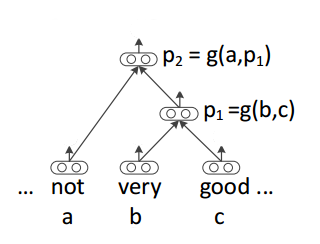
\includegraphics[scale=0.7]{rntn}
\caption{\textbf{Рекурсивная тензорная нейронная сеть}}
\label{fig:rntn}
\end{figure}
 